\section{Definitionsphase}

% Neurowissenschaftliche Grundlagen
\subsection{Theoretische Grundlagen}
% Nochmal drüber lesen
\subsubsection{Lernen ist nicht gleich Verstehen}
Im Alltag werden die Begriffe \gqq{Lernen} und \gqq{Verstehen} oft synonym verwendet. In der Wissenschaft werden diese Begriffe jedoch unterschiedlich definiert. \gqq{\textbf{Lernen}} ist ein Prozess, bei welchem Wissen, Emotionen, Fertigkeiten, aber auch Verhalten, Einstellungen und Werte durch Erfahrungen verändert werden. Hierbei werden neue Informationen erfasst und im Gehirn gespeichert, wobei das Verständnis noch nicht voll ausgereift ist. \cite*{maier_definition_lernen_nodate} \newline

\noindent
Beim Erlernen neuer Informationen treffen diese zuerst auf den Hippocampus des Gehirns und lösen dort ein Aktivitätsmuster der Nervenzellen aus. Dabei wird durch dieses Erregunsmuster entschieden, ob das neue Wissen an das Großhirn weitergeleitet wird. Nachdem die wichtigsten Informationen aufgenommen wurden, müssen die Teile in der Großhirnrinde trainiert werden, damit das Netzwerk die Möglichkeit hat, die Kontaktstellen anzupassen. Das bedeutet je öfter eine Information erneut erlernt wird, desto tiefer verankert sich diese im Langzeitgedächtnis. Im Gegenzug kann das erlangte Wissen auch verblassen, wenn die Nervenzellen nicht länger stimuliert werden. \cite[27]{beck_das_neue_lernen_heißt_verstehen} \newline

\noindent
\gqq{\textbf{Verstehen}} hingegen bedeutet, dass ein Mensch ein Konzept erstellt und dieses somit auf unbekannte Fragen und neue Situationen anwenden kann. \cite[86]{beck_das_neue_lernen_heißt_verstehen} Das heiß´t, dass beim Verstehungsprozess sich neue Infos nicht gemerkt werden sollen, sondern dass die Informationen neu verarbeitet werden und somit ein tieferes Verständnis entsteht. \cite[113]{beck_das_neue_lernen_heißt_verstehen} Bei dem Verstehungsprozess kann es einen \gqq{Aha-Moment} geben, wodurch das Verständnis plötzlich eintritt und das Denkmodell sich neu formt. Somit ist das Aufbauen eines Denkmodells für das Verstehen entscheidend. \cite[114-115]{beck_das_neue_lernen_heißt_verstehen} \newline 
\subsubsection{Synapsen und deren Rolle im Lernprozess}
Synapsen sind essentiell für die Informationsverarbeitung im Gehirn und spielen eine zentrale Rolle im Lernprozess \cite{Kandel2012}. Sie sind die Verbindungen zwischen den Neuronen und ermöglichen die Informationsübertragung und -verarbeitung. Eine Synapse besteht aus einem präsynaptischen Endknopf, der Neurotransmitter in den synaptischen Spalt freisetzt, einem synaptischen Spalt, der den Raum zwischen den Neuronen darstellt, und einer postsynaptischen Dichte, die Neurotransmitter aufnimmt und den postsynaptischen Impuls auslöst \cite{Bear2015}.\newline
Das Lernen auf zellulärer Ebene involviert die Änderung der Stärke dieser synaptischen Verbindungen, ein Prozess, der als synaptische Plastizität bezeichnet wird. Die synaptische Plastizität ermöglicht es dem Gehirn, auf Erfahrungen zu reagieren und zu lernen, und wird oft mit dem Sprichwort \gqq{Neurons that fire together, wire together} umschrieben \cite{Hebb1949}. \newline
Es gibt zwei Haupttypen der synaptischen Plastizität: Long-Term Potentiation (LTP) und Long-Term Depression (LTD). LTP erhöht die Stärke synaptischer Verbindungen und ist eng mit dem Prozess des Lernens und der Gedächtnisbildung verbunden. Auf der anderen Seite verringert LTD die Stärke der Verbindungen und wird mit dem Löschen unnötiger oder fehlerhafter Informationen assoziiert \cite{Cooke2006}. \newline
Ein interessanter Aspekt der synaptischen Plastizität ist die Tatsache, dass sie Aktivitätsabhängig ist. Das bedeutet, dass Veränderungen in der Stärke synaptischer Verbindungen nicht zufällig auftreten, sondern auf das Vorhandensein spezifischer Muster neuronaler Aktivität reagieren \cite{Kandel2012}. Dieses Phänomen erklärt, warum bestimmte Lernerfahrungen stärkere und dauerhaftere Spuren in unserem Gedächtnis hinterlassen als andere. \newline
Die Fähigkeit von Synapsen, ihre Stärke und Struktur zu ändern, bildet die Grundlage für die Anpassungsfähigkeit und Flexibilität unseres Gehirns und ermöglicht es uns, ein Leben lang zu lernen und uns an neue Erfahrungen anzupassen \cite{Bear2015}. \newline

\subsubsection{Neuronen: Die Bausteine des Gehirns}
Neuronen sind die grundlegenden funktionellen Einheiten des Gehirns und des Nervensystems. Sie sind spezialisiert auf das Senden, Empfangen und Verarbeiten von Informationen und bilden ein komplexes Netzwerk, das als Grundlage für alle kognitiven Funktionen, einschließlich Lernen und Gedächtnis, dient \cite{Bear2015}. \newline
Ein typisches Neuron besteht aus drei Hauptkomponenten: dem Zellkörper (auch Soma genannt), den Dendriten und dem Axon. Der Zellkörper enthält den Kern der Zelle und andere lebenswichtige Organellen. Die Dendriten sind verzweigte Fortsätze, die Signale von anderen Neuronen empfangen, und das Axon ist ein langer Fortsatz, der Signale an andere Neuronen weiterleitet \cite{Kandel2012}. \newline
Die Übertragung von Informationen zwischen Neuronen findet in spezialisierten Verbindungen namens Synapsen statt. Wenn ein Signal das Ende des Axons erreicht, wird ein chemischer Neurotransmitter freigesetzt, der die synaptische Verbindung überquert und ein Signal in der nachfolgenden Neuronenzelle auslöst \cite{Bear2015}. \newline
Laut Manfred Spitzer ist das Neuron nicht nur ein einfacher Signalüberträger, sondern spielt auch eine aktive Rolle in Lernprozessen \cite{Spitzer2002}. Neuronen können ihre Aktivität und Vernetzung in Abhängigkeit von der erhaltenen Information modifizieren. Das bedeutet, dass der Lernprozess nicht nur die Stärkung bestehender neuronalen Verbindungen beinhaltet, sondern auch die Bildung neuer Verbindungen und den Abbau unnötiger Verbindungen. Dieser dynamische und anpassungsfähige Charakter des neuronalen Netzwerks bildet die Grundlage für unsere Fähigkeit, ein Leben lang zu lernen und uns an ständig wechselnde Umstände anzupassen \cite{Spitzer2002}. \newline
\subsubsection{Neuronale Netze: Die Grundlage des Lernens und des Gedächtnisses}
Ein neuronales Netz ist ein komplexes System von miteinander verbundenen Neuronen, das Informationen verarbeiten und speichern kann. In seiner einfachsten Form besteht ein neuronales Netz aus einer Eingangsschicht (den Dendriten), einer oder mehreren versteckten Schichten (den Neuronen) und einer Ausgangsschicht (den Axonen) \cite{Bear2015}. \newline
Neuronale Netze sind hochdynamisch und anpassungsfähig. Sie ändern ihre Struktur und Funktion in Abhängigkeit von den Informationen, die sie erhalten, ein Prozess, der als synaptische Plastizität bezeichnet wird \cite{Kandel2012}. Dies ermöglicht es uns, zu lernen und uns an wechselnde Umgebungen und Erfahrungen anzupassen. \newline
Manfred Spitzer beschreibt, dass diese Flexibilität der neuronalen Netze es uns ermöglicht, komplexe kognitive Fähigkeiten wie Gedächtnis, Lernen, Aufmerksamkeit und Emotionen zu entwickeln \cite{Spitzer2002}. Im Gegensatz zu einem Computer, der auf festen Algorithmen basiert, kann unser Gehirn seine Struktur und Funktion an die Anforderungen der Umwelt anpassen. Dies ermöglicht es uns, ein Leben lang zu lernen und uns an neue Situationen anzupassen. \newline
Es ist wichtig zu beachten, dass, obwohl die Metapher des neuronalen Netzwerks hilft, die Funktion des Gehirns zu erklären, sie die Komplexität und Feinheit des tatsächlichen biologischen Systems nicht vollständig einfängt. Die Beziehungen zwischen Neuronen sind nicht einfach binär, sondern beinhalten eine Vielzahl von Neurotransmittern und Mechanismen, die eine fein abgestimmte Kontrolle und Modulation der neuronalen Aktivität ermöglichen \cite{Cooke2006}. \newline
Trotz dieser Einschränkungen bleibt das Modell des neuronalen Netzwerks ein mächtiges Werkzeug, um zu verstehen, wie unser Gehirn Informationen verarbeitet und speichert, und bildet die Grundlage für viele Ansätze in der kognitiven Psychologie und der künstlichen Intelligenz \cite{Hebb1949}. \newline
\newpage
\subsubsection{Optimaler Lernplan anhand des Spacing Effect}
\gqq{Das neue Lernen heißt verstehen} von Ulrich Beck vergleicht dieser das langfristige Lernen mit dem gießen einer Blume. Hierbei ist es wichtig, dass die Blumen in regelmäßigen Abständen gegossen werden, anstatt sie einmal mit einer großen Menge Wasser zu gießen. Bei den Menschen ist dies ähnlich. Viele lernen den ganzen Tag und versuchen so viel wie möglich in kurzer Zeit zu lernen, was jedoch nicht effektiv ist, da das Gehirn nicht in der Lage ist, so viel auf einmal zu verarbeiten und dieses Wissen nach einer Prüfung wieder vergessen wird. \cite[159]{beck_das_neue_lernen_heißt_verstehen} \newline

\noindent
Dadurch ist es wichtig Pausen zwischen dem Lernen einzulegen, damit das Gehirn die Informationen verarbeiten kann. Dieser Effekt wird auch \gqq{Spacing Effect} genannt und wurde von dem deutschen Psychologen und Pionier der Gedächtnisforschung Hermann Ebbinghaus entdeckt. \cite{spacing_effect} Die größten Entdeckungen waren im Bereich des Vergessens und des Lernens. Im folgenden Diagramm \ref*{fig:EbbinghausVergesseneskurve} ist die Kurve des Vergessens von Ebbinghaus dargestellt. Hierbei ist zu erkennen, dass nach einer Stunde bereits 50\% des Wissens vergessen wurde. Nach einem Tag sind nur noch 20\% des gelernten Wissens vorhanden.
\begin{figure}[H]
  \centering
  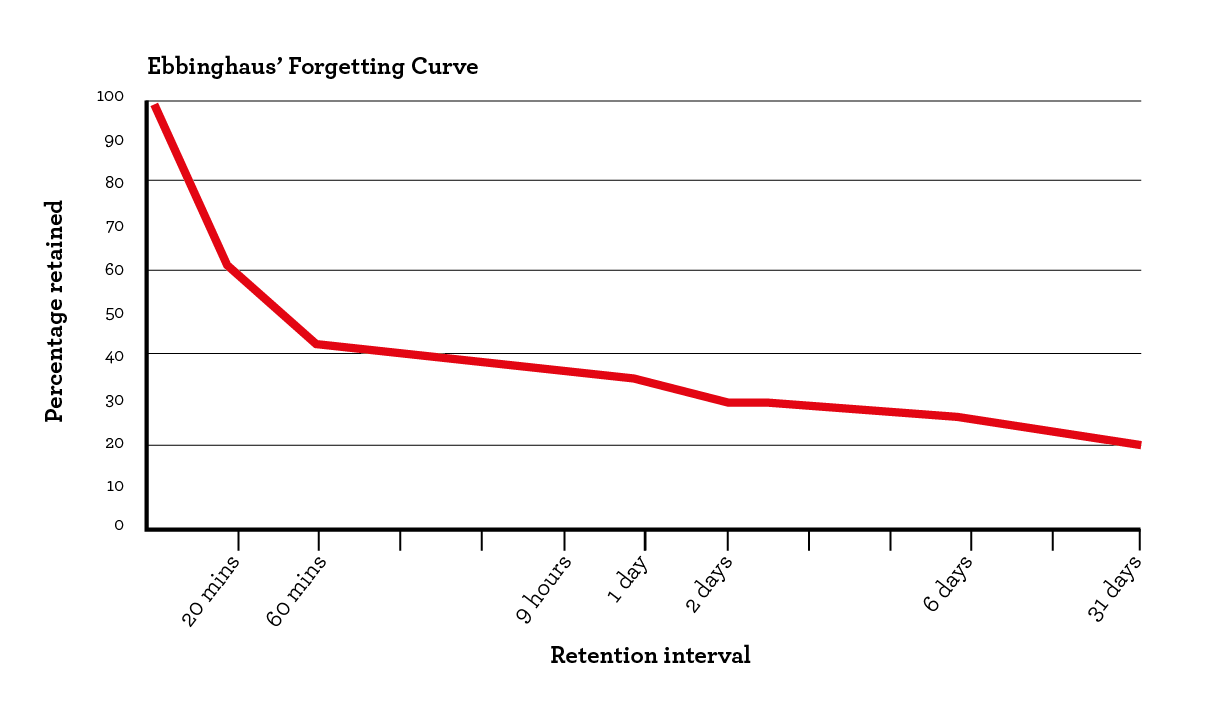
\includegraphics[width=1\textwidth]{images/diagramme/Forgetting_Curve.png}
  \caption{Ebbinghaus Vergessenskurve}
  \label{fig:EbbinghausVergesseneskurve}
\end{figure}

\newpage
\noindent
Durch das regelmäßige Wiederholen des gelernten Wissens kann die Vergessenskurve verzögert werden. Im folgenden Diagramm \ref*{fig:EbbinghausVerzoegerteVergesseneskurve} wird verdeutlicht, dass durch das Wiederholen des Wissens die Kurve des Vergessens verzögert wird. Hierbei besteht die Möglichkeit, dass nach der dritten Wiederholung das Wissen nach 60 Tagen noch zu 90\% vorhanden ist. \cite*{spacing_effect} Der Abstand der Wiederholungen bezieht sich hierbei darauf, dass erst wieder der Stoff gelernt wird, wenn dieser nur noch eine 90 prozentige Chance hat, vorhanden zu sein. Hierdurch wird klargestellt, dass das Wiederholen des Stoffes wichtig ist, um das Wissen langfristig beizubehalten. \newline

\begin{figure}[H]
  \centering
  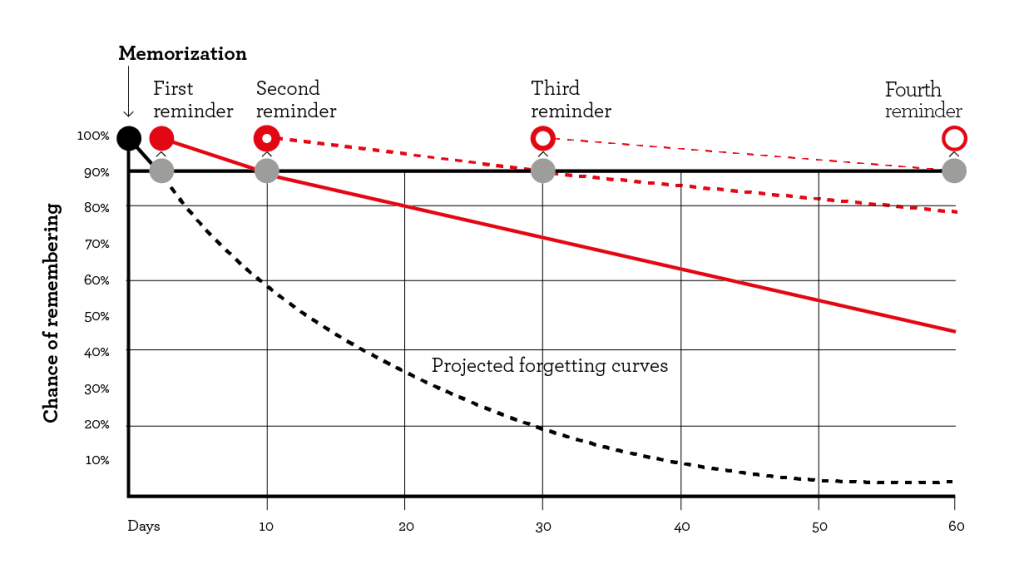
\includegraphics[width=1\textwidth]{images/diagramme/Delayed_Forgetting_Curve.png}
  \caption{Ebbinghaus verzögerte Vergessenskurve durch Wiederholungen}
  \label{fig:EbbinghausVerzoegerteVergesseneskurve}
\end{figure}

\noindent
Die Daumenregel für die optimale Pausenlänge beträgt 10 - 20\% der Zeit, bis diese Information angewendet werden muss. Wenn beispielsweise eine Prüfung in 30 Tagen stattfindet, sollte der Stoff alle 3 - 6 Tage wiederholt werden. \cite[160]{beck_das_neue_lernen_heißt_verstehen}  Dieser Fall kann beschrieben werden: 
\[ \text{{Pausenlänge}} = (\text{{30 Tage}}) \times (0.1 - 0.2) \]
\noindent
Die allgemeine Formel könnte man beschreiben als: 
\[ \text{{Pausenlänge}} = (\text{{Zeit bis zur Anwendung}}) \times (0.1 - 0.2) \]
\newpage
\noindent
Aus dieser Formel kann abgeleitet werden, dass zwischen fünf und zehn Wiederholungen notwendig sind, um das Wissen langfristig zu behalten. \cite[160]{beck_das_neue_lernen_heißt_verstehen} Mit diesen Informationen kann ein optimaler Lernplan erstellt werden, der die Wiederholungen automatisch berechnet und den Nutzer daran erinnert, wann er wieder lernen muss.

\subsubsection{Tagging innerhalb der Lern-App}
%ToDo Tagging Begriff ins Glossar
Um den Benutzer:in das Lernen so einfach wie möglich zu gestalten wurde entschieden, dass dieser die Möglichkeit hat, bestimmte Lerninhalte zu taggen. Das Verwenden von Tags wird in den folgenden Funktionen der App ermöglicht:
\begin{itemize}
  \item Fragen erstellen
  \item Test erstellen
  \item Zusammenfassungen erstellen
  \item Lernhilfe bei beantworten fehlerhafter Fragen
\end{itemize}

\noindent
Wenn ein Nutzer eine \textbf{Frage erstellen} möchte, dann muss die neu erstellte Frage mindestens einen Tag besitzen. Es ist möglich, dass eine Frage mehrere Tags enthalten darf. \newline

\noindent
Wenn ein Nutzer einen \textbf{Test erstellen} möchte, dann hat dieser die Option, eine Frage manuell oder mehrere Fragen anhand von Tags hinzufügen zu können. Hierbei werden alle Fragen, die den gewählten Tag beinhalten, dem Test zugeordnet. Dies vereinfacht das Erstellen eines Tests, da der Nutzer nicht jede Frage einzeln hinzufügen muss. \newline

\noindent
In der Lern-App kann der Nutzer mithilfe eines Editors eine \textbf{Zusammenfassung erstellen}. Dieser soll grundsätzlich die gleichen Funktionen wie andere gängige Texteditoren besitzen. Das heißt im genaueren Sinne, dass der Nutzer die Option hat, seinen Text zu formatieren, Bilder sowie Links einzufügen und den Text zu speichern. Zusätzlich soll es möglich sein, dass ein Text mit einem Tag versehen werden kann. \newline 

\noindent
Wenn ein Anwender eine Frage hintereinander mehrfach falsch beantwortet, dann soll anhand des Tags eine \textbf{Lernhilfe} angeboten werden. Hierbei wird der Nutzer gefragt, ob dieser sich den Teil der Zusammenfassung nochmal anschauen möchte. Dabei ist es erforderlich, dass in der Zusammenfassung mindestens ein Tag dieser Frage vorhanden ist. Wenn der Nutzer sich die Zusammenfassung anschauen möchte, dann soll der Tag als Sprungmarke dienen und den Nutzer direkt zu dem zugehörigen Teil der Zusammenfassung weterleiten. \newline 

\subsubsection{Lernkategorien \& Lernziele}
Um dem Benutzer die einfache Kategorisierung und Planung seiner Lerninhalte zu ermöglichen gibt es die Möglichkeit Lernkategorien und Lernziele zu erstellen. \newline
Im Reiter \gqq{Lernkategorien} können Lernkategorien erstellt werden. Eine Lernkategorie besteht aus
\begin{itemize}
  \item Zusammenfassungen
  \begin{itemize}
    \item Eine Zusammenfassung muss vom Benutzer erstellt werden und bietet mithilfe von \gqq{Markdown} (\href{https://www.markdownguide.org/basic-syntax}{Siehe Markdown Guide}) die Möglichkeit Informationen strukturiert darzustellen.
  \end{itemize}
  \item Tests/Fragen
  \begin{itemize}
    \item Eine Frage muss vom Benutzer erstellt werden und besitzt auch eine zugehörige Antwort. Jede Frage besitzt einen Fragentyp, der die Form der Frage definiert und wie diese den Benutzer abfragt. In der bisherigen Version der App werden nur Fragen vom Karteikarten-Fragetyp unterstützt. Eine Ansammlung von Fragen kann zu einem Test zusammengefasst und somit gruppiert abgefragt werden.
  \end{itemize}
\end{itemize}
\subsubsection{Gamification und ihr positiver Effekt auf das Lernen}
Gamification bezeichnet die Anwendung von Spielelementen in nicht-spielerischen Kontexten, um Motivation und Engagement zu steigern \cite{Deterding2011}. Im Bildungsbereich hat die Gamification-Strategie zunehmend an Popularität gewonnen, da sie das Lernen attraktiver und interaktiver gestaltet \cite{Hamari2014}.\newline
Durch die Einbeziehung von Spielelementen wie Punkten, Leveln, Belohnungen, Herausforderungen und Leaderboards wird der Lernprozess in einen Wettbewerbs- und Unterhaltungskontext eingebettet \cite{Kapp2012}. Dies kann dazu beitragen, die Motivation der Lernenden zu erhöhen, was wiederum zu einer höheren Teilnahme und verbesserten Lernergebnissen führen kann \cite{Hanus2015}.\newline
Ein weiterer Vorteil der Gamification ist, dass sie durch Feedback und Belohnungen eine unmittelbare Rückmeldung zum Lernprozess ermöglicht. Dies kann dazu beitragen, die Selbstwirksamkeit der Lernenden zu erhöhen und ein Gefühl der Leistung und des Fortschritts zu fördern \cite{Landers2014}. \newline
Trotz der potenziellen Vorteile ist es wichtig, die Gamification sorgfältig zu gestalten und durchzuführen. Eine schlecht durchdachte Gamification kann zu einer Überbetonung von Wettbewerb und Leistung führen, was wiederum zu Stress und Angst bei den Lernenden führen kann \cite{Nicholson2015}. Daher ist es wichtig, ein ausgewogenes Gleichgewicht zwischen Wettbewerb und Zusammenarbeit, Belohnung und Herausforderung zu schaffen, um ein gesundes und effektives Lernumfeld zu gewährleisten \cite{Deterding2011}.\newline
Bei LearnAhead wird die Gamification mit einem Punktesystem umgesetzt. Beim Lernen bekommt der Benutzer direktes Feedback und erhöht somit seine eigene Punktzahl. Punkte werden auf dem Profil angezeigt und mit folgenden Ereignissen verdient.
\begin{itemize}
  \item Abschliessen eines Tests - 10 Punkte
  \item Einloggen an einem neuen Tag - zwischen 10 und 100 Punkte, je nach Anzahl der sequentiell aufeinanderfolgenden Einlogg-Tage
  \item Erreichen eines Lernziels - 20 Punkte
\end{itemize}
\subsection{Pflichtenheft}
Das Pflichtenheft ist analog zum
\hyperref[sec:arbeitspaketplan]{Arbeitspaketplan} in diesem Dokument nicht
genauer beschrieben, sondern in Form eines Backlog auf
\href{https://studienarbeitlernapp.atlassian.net/jira/software/projects/LER/boards/1}{\underline{Jira}}\footnote{\href{https://studienarbeitlernapp.atlassian.net/jira/software/projects/LER/boards/1}{https://studienarbeitlernapp.atlassian.net/jira/software/projects/LER/boards/1}}
aufgeführt. Dort kann entweder der Reiter \gqq{Roadmap} oder der Reiter
\gqq{Board} aufgerufen werden.

\subsection{Use Case Diagramm}

\begin{figure}[H]
  \centering
  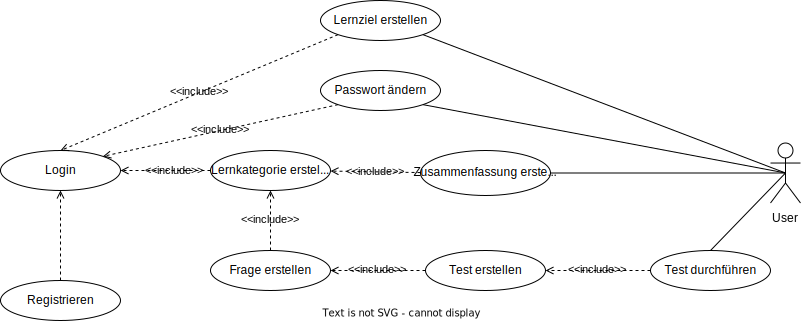
\includegraphics[width=1\textwidth]{images/diagramme/UseCase_Diagramm.png}
  \caption{Use Case Diagramm}
  \label{fig:UseCaseDiagramm}
\end{figure}
\newpage
\subsection{Use Case Beschreibung}

% Use Case Login
\begin{table}[h!]
  \begin{tabular}{p{0.2\textwidth}|p{0.74\textwidth}}
    \textbf{Name:}     & \textbf{Login}                                                                  \\ \hline
    Ziel:              & Anmelden mit bestehenden Logindaten in der App                                  \\ \hline
    Kategorie:         & Primär                                                                          \\ \hline
    Vorbedingung:      & Der Benutzer muss bereits einen Account erstellt haben                          \\ \hline
    Nachbedingung:     & Der Benutzer ist eingeloggt                                                     \\ \hline
    Fehlerfälle:       &
    \begin{minipage}[t]{\linewidth}
      Falsche Logindaten
      \strut
      \begin{itemize}
        \item Rückmeldung, dass falsche Zugangsdaten verwendet wurden
        \item Möglichkeit, das Kennwort über die E-Mail zurückzusetzen
      \end{itemize}
      Abbruch durch den Benutzer
      \begin{itemize}
        \item keine Zustandsänderung \strut
      \end{itemize}
    \end{minipage}                                                                       \\ \hline
    Akteure:           & User                                                                            \\ \hline
    Auslösendes Event: & Benutzer öffnet die App und klickt auf einloggen                                \\ \hline
    Beschreibung/
    Erweiterungen:     & Der Benutzer meldet sich an, um die verschiedenen Dienste der App zu verwenden  \\ \hline
    Alternativen:      & Benutzer kann sich registrieren, sofern die E-Mail nicht schon registriert ist. \\
  \end{tabular}
\end{table}
% Use Case Registrieren
\begin{table}[h!]
  \begin{tabular}{p{0.2\textwidth}|p{0.74\textwidth}}
    \textbf{Name:}     & \textbf{Registrieren}                                       \\ \hline
    Ziel:              & Anlegen eines neuen Accounts                                \\ \hline
    Kategorie:         & Primär                                                      \\ \hline
    Vorbedingung:      & E-Mail ist noch nicht mit einem anderen Account registriert \\ \hline
    Nachbedingung:     & Der Benutzer ist eingeloggt                                 \\ \hline
    Fehlerfälle:       &
    \begin{minipage}[t]{\linewidth}
      E-Mail bereits verwendet
      \strut
      \begin{itemize}
        \item Rückmeldung, dass E-Mail bereits verwendet wurde
      \end{itemize}
      Abbruch durch den Benutzer
      \begin{itemize}
        \item Keine Zustandsänderung
        \item Account wird nicht angelegt \strut
      \end{itemize}
    \end{minipage}                                                   \\ \hline
    Akteure:           & User                                                        \\ \hline
    Auslösendes Event: & Benutzer öffnet die App und klickt auf Registrieren.        \\ \hline
    Beschreibung/
    Erweiterungen:     & Ein Benutzer möchte einen neuen Account erstellen.          \\ \hline
    Alternativen:      & Login mit bestehendem Account.                              \\
  \end{tabular}
\end{table}
% Use Case Lernziel erstellen
\begin{table}[h!]
  \begin{tabular}{p{0.2\textwidth}|p{0.74\textwidth}}
    \textbf{Name:}     & \textbf{Lernziel erstellen}                                                                                                                                                \\ \hline
    Ziel:              & Anlegen eines neuen Lernziels                                                                                                                                              \\ \hline
    Kategorie:         & Primär                                                                                                                                                                     \\ \hline
    Vorbedingung:      &
    \begin{minipage}[t]{\linewidth}
      \strut
      \begin{itemize}
        \item User musss eingeloggt sein
        \item Lernziel mit gleichem Namen ist noch nicht erstellt \strut
      \end{itemize}
    \end{minipage}                                                                                                                                                                  \\ \hline
    Nachbedingung:     & Lernziel ist erstellt                                                                                                                                                      \\ \hline
    Fehlerfälle:       &
    \begin{minipage}[t]{\linewidth}
      Lernziel mit gleichem Namen existiert bereits
      \strut
      \begin{itemize}
        \item Rückmeldung, dass dieses Lernziel bereits existiert
      \end{itemize}
      Abbruch durch den Benutzer
      \begin{itemize}
        \item keine Zustandsänderung
        \item Lernziel wird nicht angelegt \strut
      \end{itemize}
    \end{minipage}                                                                                                                                                    \\ \hline
    Akteure:           & User                                                                                                                                                                       \\ \hline
    Auslösendes Event: & Benutzer öffnet Lernziel Reiter und klickt auf \gqq{Lernziel erstellen}                                                                                                    \\ \hline
    Beschreibung/
    Erweiterungen:     & Durch das Ausfüllen der Eingabefelder und anschließendes bestätigen, kann der User ein Lernziel erstellen. Aus sämtlichen Lernzielen wird daraufhin ein Lernplan erstellt. \\ \hline
    Alternativen:      &                                                                                                                                                                            \\
  \end{tabular}
\end{table}
% Use Case Lernkategorie erstellen
\begin{table}[H]
  \begin{tabular}{p{0.2\textwidth}|p{0.74\textwidth}}
    \textbf{Name:}     & \textbf{Lernkategorie erstellen}                                                                                                                                                                         \\ \hline
    Ziel:              & Anlegen einer neuen Lernkategorie                                                                                                                                                                   \\ \hline
    Kategorie:         & Primär                                                                                                                                                                                              \\ \hline
    Vorbedingung:      &
    \begin{minipage}[t]{\linewidth}
      \strut
      \begin{itemize}
        \item User musss eingeloggt sein
        \item Lernkategorie mit gleichem Namen ist noch nicht erstellt \strut
      \end{itemize}
    \end{minipage}                                                                                                                                                                                           \\ \hline
    Nachbedingung:     & Lernkategorie ist erstellt                                                                                                                                                                          \\ \hline
    Fehlerfälle:       &
    \begin{minipage}[t]{\linewidth}
      Lernkategorie mit gleichem Namen existiert bereits
      \strut
      \begin{itemize}
        \item Rückmeldung, dass diese Lernkategorie bereits existiert
      \end{itemize}
      Abbruch durch den Benutzer
      \begin{itemize}
        \item keine Zustandsänderung
        \item Lernkategorie wird nicht angelegt \strut
      \end{itemize}
    \end{minipage}                                                                                                                                                                        \\ \hline
    Akteure:           & User                                                                                                                                                                                                \\ \hline
    Auslösendes Event: & Benutzer öffnet Lernkategorie Reiter und klickt auf \gqq{Lernkategorie erstellen}                                                                                                                   \\ \hline
    Beschreibung/
    Erweiterungen:     & Durch das Ausfüllen der Eingabefelder und anschließendes bestätigen, kann der User eine Lernkategorie erstellen. In einer Lernkategorie können Zusammenfassungen, Fragen und Tests erstellt werden. \\ \hline
    Alternativen:      &                                                                                                                                                                                                     \\
  \end{tabular}
\end{table}
% Use Case Zusammenfassung erstellen
\begin{table}[h!]
  \begin{tabular}{p{0.2\textwidth}|p{0.74\textwidth}}
    \textbf{Name:}     & \textbf{Zusammenfassung erstellen}                                                                                                                                                          \\ \hline
    Ziel:              & Anlegen einer neuen Zusammenfassung                                                                                                                                                         \\ \hline
    Kategorie:         & Primär                                                                                                                                                                                      \\ \hline
    Vorbedingung:      &
    \begin{minipage}[t]{\linewidth}
      \strut
      \begin{itemize}
        \item User musss eingeloggt sein
        \item Zusammenfassung mit gleichem Namen ist noch nicht in der gleichen Lernkategorie
              erstellt \strut
      \end{itemize}
    \end{minipage}                                                                                                                                                                                   \\ \hline
    Nachbedingung:     & Zusammenfassung für Lernkategorie ist erstellt                                                                                                                                              \\ \hline
    Fehlerfälle:       &
    \begin{minipage}[t]{\linewidth}
      Zusammenfassung mit gleichem Namen existiert bereits in dieser Lernkategorie
      \strut
      \begin{itemize}
        \item Rückmeldung, dass diese Zusammenfassung bereits existiert
      \end{itemize}
      Abbruch durch den Benutzer
      \begin{itemize}
        \item keine Zustandsänderung
        \item Zusammenfassung wird nicht angelegt \strut
      \end{itemize}
    \end{minipage}                                                                                                                                      \\ \hline
    Akteure:           & User                                                                                                                                                                                        \\ \hline
    Auslösendes Event: & Benutzer öffnet eine Lernkategorie, klickt auf \gqq{Zusammenfassungen} und danach auf \gqq{Zusammenfassung erstellen}                                                                       \\ \hline
    Beschreibung/
    Erweiterungen:     & Durch das Ausfüllen der Eingabefelder und anschließendes bestätigen, kann der User eine Zusammenfassung erstellen. In einer Zusammenfassung können Inhalte eingefügt und formatiert werden. \\ \hline
    Alternativen:      &                                                                                                                                                                                             \\
  \end{tabular}
\end{table}
% Use Case Frage erstellen
\begin{table}[H]
  \begin{tabular}{p{0.2\textwidth}|p{0.74\textwidth}}
    \textbf{Name:}     & \textbf{Frage erstellen}                                                                                                                                                                                                                                               \\ \hline
    Ziel:              & Anlegen einer neuen Frage                                                                                                                                                                                                                                              \\ \hline
    Kategorie:         & Primär                                                                                                                                                                                                                                                                 \\ \hline
    Vorbedingung:      &
    \begin{minipage}[t]{\linewidth}
      \strut
      \begin{itemize}
        \item User musss eingeloggt sein
        \item Frage mit gleichem Index ist noch nicht in der gleichen Lernkategorie erstellt
              \strut
      \end{itemize}
    \end{minipage}                                                                                                                                                                                                                                                              \\ \hline
    Nachbedingung:     & Frage für Lernkategorie ist erstellt                                                                                                                                                                                                                                   \\ \hline
    Fehlerfälle:       &
    \begin{minipage}[t]{\linewidth}
      Frage mit gleichem Namen existiert bereits in dieser Lernkategorie
      \strut
      \begin{itemize}
        \item Rückmeldung, dass Frage mit gleicher Bezeichnung bereits existiert
      \end{itemize}
      Abbruch durch den Benutzer
      \begin{itemize}
        \item keine Zustandsänderung
        \item Frage wird nicht angelegt \strut
      \end{itemize}
    \end{minipage}                                                                                                                                                                                                                           \\ \hline
    Akteure:           & User                                                                                                                                                                                                                                                                   \\ \hline
    Auslösendes Event: & Benutzer öffnet eine Lernkategorie, klickt auf \gqq{Tests / Fragen} und danach auf \gqq{Frage erstellen}                                                                                                                                                               \\ \hline
    Beschreibung/
    Erweiterungen:     & Durch das Ausfüllen der Eingabefelder und anschließendes bestätigen, kann der User eine Frage erstellen. Eine Frage kann unterschiedliche Vorlagen (beispielsweise Karteikarte) besitzen, jedoch gibt es immer eine Meldung (Text der Frage) und eine gültige Antwort. \\ \hline
    Alternativen:      &                                                                                                                                                                                                                                                                        \\
  \end{tabular}
\end{table}
% Use Case Test erstellen
\begin{table}[H]
  \begin{tabular}{p{0.2\textwidth}|p{0.74\textwidth}}
    \textbf{Name:}     & \textbf{Test erstellen}                                                                                                                                                                                                                                                                           \\ \hline
    Ziel:              & Anlegen eines neuen Tests                                                                                                                                                                                                                                                                         \\ \hline
    Kategorie:         & Primär                                                                                                                                                                                                                                                                                            \\ \hline
    Vorbedingung:      &
    \begin{minipage}[t]{\linewidth}
      \strut
      \begin{itemize}
        \item User musss eingeloggt sein
        \item Test mit gleichem Namen ist noch nicht in der gleichen Lernkategorie erstellt
              \strut
      \end{itemize}
    \end{minipage}                                                                                                                                                                                                                                                                                         \\ \hline
    Nachbedingung:     & Test für Lernkategorie ist erstellt                                                                                                                                                                                                                                                               \\ \hline
    Fehlerfälle:       &
    \begin{minipage}[t]{\linewidth}
      Test mit gleichem Namen existiert bereits in dieser Lernkategorie
      \strut
      \begin{itemize}
        \item Rückmeldung, dass Test mit gleicher Bezeichnung bereits existiert
      \end{itemize}
      Abbruch durch den Benutzer
      \begin{itemize}
        \item keine Zustandsänderung
        \item Test wird nicht angelegt \strut
      \end{itemize}
    \end{minipage}                                                                                                                                                                                                                                                       \\ \hline
    Akteure:           & User                                                                                                                                                                                                                                                                                              \\ \hline
    Auslösendes Event: & Benutzer öffnet eine Lernkategorie, klickt auf \gqq{Tests / Fragen} und danach auf \gqq{Test erstellen}                                                                                                                                                                                           \\ \hline
    Beschreibung/
    Erweiterungen:     & Durch das Ausfüllen der Eingabefelder und anschließendes bestätigen, kann der User einen Test erstellen. Eine Test kann mehrere Fragen besitzen. Wenn ein Test gestartet wird, bekommt der User nach abschließen des Tests eine Meldung, wie viele und welche Fragen er richtig beantwortet hast. \\ \hline
    Alternativen:      &                                                                                                                                                                                                                                                                                                   \\
  \end{tabular}
\end{table}
\newpage

\subsection{Datenbankstruktur}
\subsubsection{Datenbankmodell}
\begin{figure}[H]
  \centering
  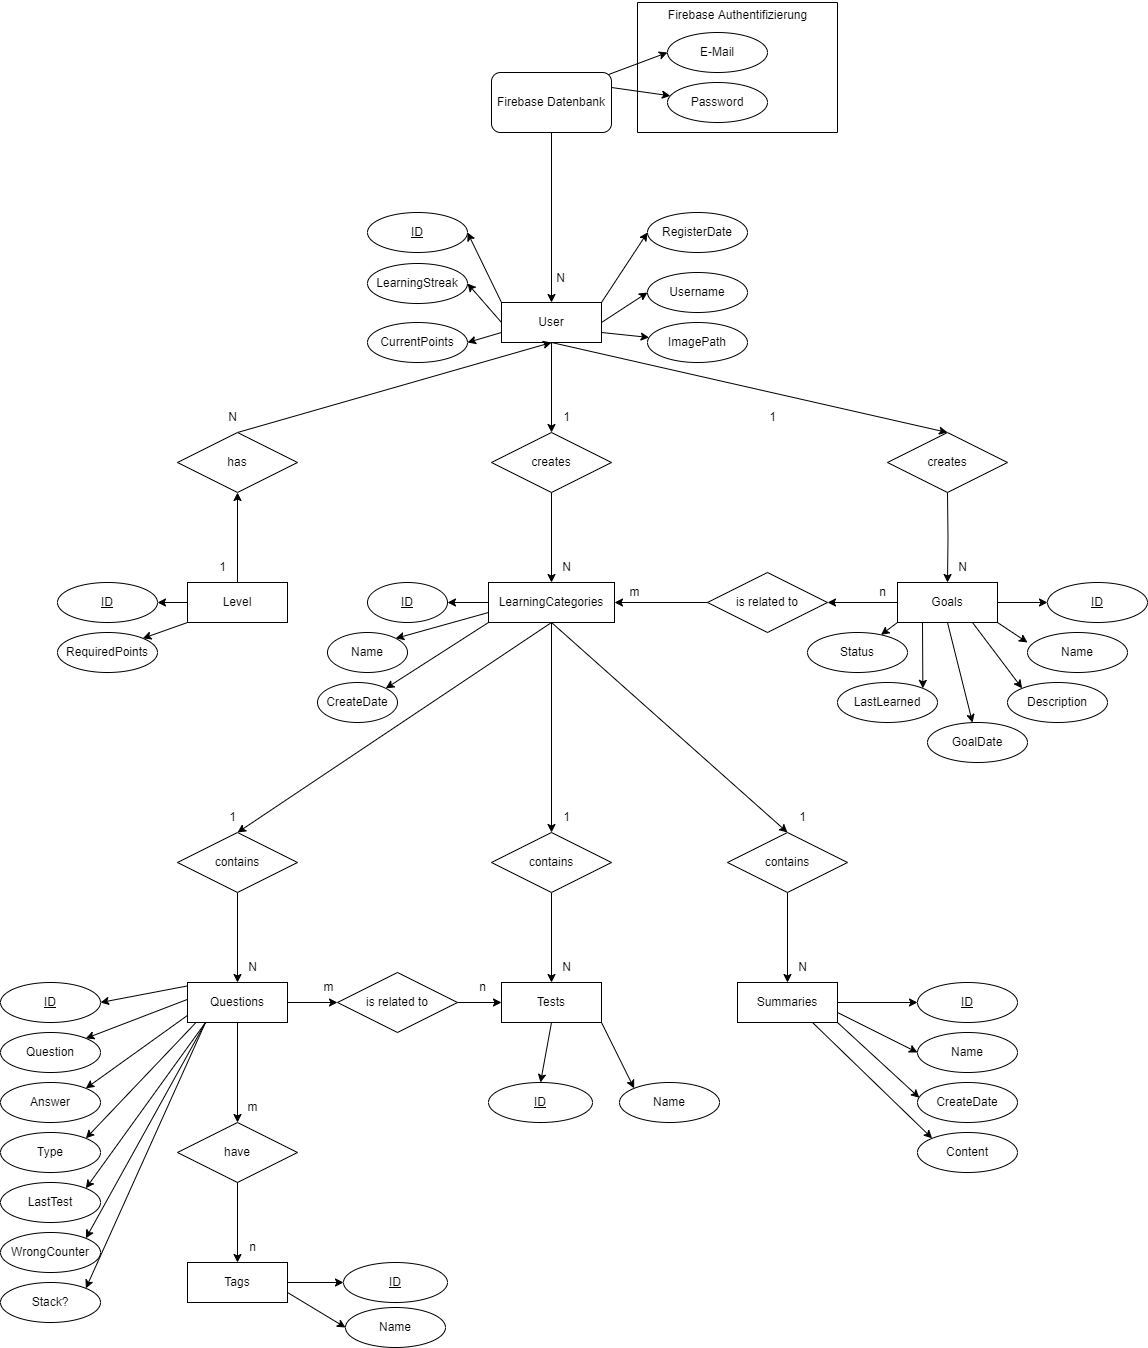
\includegraphics[width=1\textwidth]{images/LearnAheadDatenbankstruktur.png}
  \caption{LearnAhead Datenbankstruktur}
  \label{fig:LearnAheadDatenbankstruktur}
\end{figure}\noindent
\subsubsection{Data Dictionary}
\underline{\textbf{User}}
\begin{table}[H]
  \centering
  \resizebox{\columnwidth}{!}{%
    \begin{tabular}{c|c|c|c|c|c|l}
      \textbf{Attribut}  &
      \textbf{Datentyp}  &
      \textbf{Länge}     &
      \textbf{Null}      &
      \textbf{Default}   &
      \textbf{Schlüssel} &
      \textbf{Beschreibung}                                                                                                                                                         \\ \hline
      ID                 &
      string             &
      -                  &
      Nein               &
      -                  &
      P                  &
      \\ \hline
      Username           &
      string             &
      -                  &
      Nein               &
      -                  &
      -                  &
      Der Benutzername des Nutzers                                                                                                                                                  \\ \hline
      E-Mail             &
      string             &
      -                  &
      Nein               &
      -                  &
      -                  &
      Die E-Mail-Adresse des Nutzers                                                                                                                                                \\ \hline
      Password           &
      string             &
      -                  &
      Nein               &
      -                  &
      -                  &
      Das Passwort des Nutzers                                                                                                                                                      \\ \hline
      ProfileImageURL    &
      string             &
      -                  &
      Ja                 &
      Null               &
      -                  &
      \begin{tabular}[c]{@{}l@{}}Der Link des Profilbilds welches\\ im Firebase Storage gespeichert\\ ist\end{tabular}                                                              \\ \hline
      RegisterDate       &
      timestamp          &
      -                  &
      Nein               &
      -                  &
      -                  &
      \begin{tabular}[c]{@{}l@{}}Das Datum an dem sich der \\ Nutzer registriert hat.\end{tabular}                                                                                  \\ \hline
      LearningStreak     &
      number             &
      -                  &
      Ja                 &
      0                  &
      -                  &
      \begin{tabular}[c]{@{}l@{}}Dies gibt die Anzahl an, wie viele\\ Tage der Nutzer aufeinander \\ gelernt hat.\end{tabular}                                                      \\ \hline
      AchievedGoals      &
      number             &
      -                  &
      Ja                 &
      0                  &
      -                  &
      \begin{tabular}[c]{@{}l@{}}Dies gibt die Anzahl an, wie viele\\ Lernziel der Nutzer erreicht hat.\end{tabular}                                                                \\ \hline
      CurrentPoints      &
      number             &
      -                  &
      Ja                 &
      0                  &
      -                  &
      \begin{tabular}[c]{@{}l@{}}Die aktuelle Level Punkte des\\ Nutzers\end{tabular}                                                                                               \\ \hline
      LearningCategories &
      map                &
      -                  &
      Ja                 &
      Null               &
      -                  &
      \begin{tabular}[c]{@{}l@{}}Dies ist eine gemappte Liste zu\\ der Tabelle LearningCategories, \\ wo alle Lernkategorien drin sind,\\ die der Nutzer erstellt hat.\end{tabular} \\ \hline
      Goals              &
      map                &
      -                  &
      Ja                 &
      Null               &
      -                  &
      \begin{tabular}[c]{@{}l@{}}Dies ist eine gemappte Liste zu \\ der Tabelle Goals, wo alle\\ Lernziele drin sind, die der\\ Nutzer erstellt hat.\end{tabular}
    \end{tabular}%
  }
\end{table}
\underline{\textbf{Level}}
\begin{table}[H]
  \centering
  \resizebox{\columnwidth}{!}{%
  \begin{tabular}{c|c|c|c|c|c|l}
  \textbf{Attribut} &
    \textbf{Datentyp} &
    \textbf{Länge} &
    \textbf{Null} &
    \textbf{Default} &
    \textbf{Schlüssel} &
    \textbf{Beschreibung} \\ \hline
  ID &
    string &
    - &
    Nein &
    - &
    P &
     \\ \hline
  RequiredPoints & number & - & Nein & - & - & \begin{tabular}[c]{@{}l@{}}Dies gibt die benötigten\\ Punkte für das spezielle\\ Level an\end{tabular} \\ \hline
  Level &
    number &
    - &
    Nein &
    - &
    - &
    \begin{tabular}[c]{@{}l@{}}Dies gibt das spezielle \\ Level anhand der Punkte an\end{tabular}
  \end{tabular}%
  }
  \end{table}
\newpage
\underline{\textbf{Goal}}
\begin{table}[H]
  \centering
  \resizebox{\columnwidth}{!}{%
    \begin{tabular}{c|c|c|c|c|c|l}
      \textbf{Attribut}                                          &
      \textbf{Datentyp}                                          &
      \textbf{Länge}                                             &
      \textbf{Null}                                              &
      \textbf{Default}                                           &
      \textbf{Schlüssel}                                         &
      \textbf{Beschreibung}                                                                                                                                       \\ \hline
      ID                                                         &
      string                                                     &
      -                                                          &
      Nein                                                       &
      -                                                          &
      P                                                          &
      \\ \hline
      Name                                                       &
      string                                                     &
      -                                                          &
      Nein                                                       &
      -                                                          &
      -                                                          &
      Der Name des Lernziels                                                                                                                                      \\ \hline
      Description                                                &
      string                                                     &
      -                                                          &
      Ja                                                         &
      Null                                                       &
      -                                                          &
      \begin{tabular}[c]{@{}l@{}}Dies soll als Beschreibung des\\ Lernziels gelten. Hier können\\ z.B. die relevanten Themen\\ aufgelistet werden.\end{tabular}   \\ \hline
      Status                                                     &
      string                                                     &
      -                                                          &
      Ja                                                         &
      ToDo                                                       &
      -                                                          &
      \begin{tabular}[c]{@{}l@{}}Dies gibt den aktuellen Status\\ des Lernziels an.\\ Es gibt die folgende Status:\\ - ToDo\\ - In Progress\\ - Done\end{tabular} \\ \hline
      StartDate                                                  &
      timestamp                                                  &
      -                                                          &
      Ja                                                         &
      \begin{tabular}[c]{@{}c@{}}Server\\ Timestamp\end{tabular} &
      -                                                          &
      \begin{tabular}[c]{@{}l@{}}Dies gibt an, wann das \\ Lernziel startet\end{tabular}                                                                          \\ \hline
      EndDate                                                    &
      timestamp                                                  &
      -                                                          &
      Nein                                                       &
      -                                                          &
      -                                                          &
      \begin{tabular}[c]{@{}l@{}}Dies gibt an, bis wann das\\ Lernziel abgeschlossen sein\\ soll\end{tabular}                                                     \\ \hline
      LastLearned                                                &
      timestamp                                                  &
      -                                                          &
      Ja                                                         &
      Null                                                       &
      -                                                          &
      \begin{tabular}[c]{@{}l@{}}Dies gibt, wann das Lernziel\\ das letzte mal gelernt wurde.\end{tabular}
    \end{tabular}%
  }
\end{table}
\newpage
% Data Dicitonary Learning Category Table
\underline{\textbf{LearningCategory}}
\begin{table}[H]
  \centering
  \resizebox{\columnwidth}{!}{%
    \begin{tabular}{c|c|c|c|c|c|l}
      \textbf{Attribut}                                          &
      \textbf{Datentyp}                                          &
      \textbf{Länge}                                             &
      \textbf{Null}                                              &
      \textbf{Default}                                           &
      \textbf{Schlüssel}                                         &
      \textbf{Beschreibung}                                                                                                                                                \\ \hline
      ID                                                         &
      string                                                     &
      -                                                          &
      Nein                                                       &
      -                                                          &
      P                                                          &
      \\ \hline
      Name                                                       &
      string                                                     &
      -                                                          &
      Nein                                                       &
      -                                                          &
      -                                                          &
      Der Name der Lernkategorie                                                                                                                                           \\ \hline
      CreateDate                                                 &
      timestamp                                                  &
      -                                                          &
      Ja                                                         &
      \begin{tabular}[c]{@{}c@{}}Server\\ Timestamp\end{tabular} &
      -                                                          &
      \begin{tabular}[c]{@{}l@{}}Dies gibt an, wann die \\ Lernkategorie erstellt wurde\end{tabular}                                                                       \\ \hline
      Goals                                                      &
      map                                                        &
      -                                                          &
      Ja                                                         &
      Null                                                       &
      -                                                          &
      \begin{tabular}[c]{@{}l@{}}Dies ist eine gemappte Liste zu\\ der Tabelle Goal,\\ wo alle Lernziele drin sind,\\ die der Nutzer erstellt hat.\end{tabular}            \\ \hline
      Questions                                                  &
      map                                                        &
      -                                                          &
      Ja                                                         &
      Null                                                       &
      -                                                          &
      \begin{tabular}[c]{@{}l@{}}Dies ist eine gemappte Liste zu\\ der Tabelle Question, wo alle \\ Fragen drin sind, die der \\ Nutzer erstellt hat.\end{tabular}         \\ \hline
      Summaries                                                  &
      map                                                        &
      -                                                          &
      Ja                                                         &
      Null                                                       &
      -                                                          &
      \begin{tabular}[c]{@{}l@{}}Dies ist eine gemappte Liste zu\\ der Tabelle Summary, wo alle\\ Zusammenfassungen drin sind,\\ die der Nutzer erstellt hat.\end{tabular} \\ \hline
      Tests                                                      &
      map                                                        &
      -                                                          &
      Ja                                                         &
      Null                                                       &
      -                                                          &
      \begin{tabular}[c]{@{}l@{}}Dies ist eine gemappte Liste zu\\ der Tabelle Test, wo alle Tests\\ drin sind, die der Nutzer\\ erstellt hat.\end{tabular}
    \end{tabular}%
  }
\end{table}
\underline{\textbf{Summary}}
\begin{table}[H]
  \centering
  \resizebox{\columnwidth}{!}{%
  \begin{tabular}{c|c|c|c|c|c|l}
  \textbf{Attribut} &
    \textbf{Datentyp} &
    \textbf{Länge} &
    \textbf{Null} &
    \textbf{Default} &
    \textbf{Schlüssel} &
    \textbf{Beschreibung} \\ \hline
  ID &
    string &
    - &
    Nein &
    - &
    P &
     \\ \hline
  Name &
    string &
    - &
    Nein &
    - &
    - &
    \begin{tabular}[c]{@{}l@{}}Dies ist der Name einer\\ Zusammenfassung\end{tabular} \\ \hline
  CreateDate &
    timestamp &
    - &
    Nein &
    - &
    - &
    \begin{tabular}[c]{@{}l@{}}Dies ist das Erstelldatum\\ einer Zusammenfassung\end{tabular} \\ \hline
  Content & string & - & Ja & Null & - & \begin{tabular}[c]{@{}l@{}}Dies ist ist der Inhalt einer\\ Zusammenfassung im \\ Raw-Format\end{tabular}
  \end{tabular}%
  }
  \end{table}
  \newpage
  \underline{\textbf{Test}}
  % Please add the following required packages to your document preamble:
% \usepackage{graphicx}
\begin{table}[H]
  \centering
  \resizebox{\columnwidth}{!}{%
  \begin{tabular}{c|c|c|c|c|c|l}
  \textbf{Attribut} &
    \textbf{Datentyp} &
    \textbf{Länge} &
    \textbf{Null} &
    \textbf{Default} &
    \textbf{Schlüssel} &
    \textbf{Beschreibung} \\ \hline
  ID &
    string &
    - &
    Nein &
    - &
    P &
     \\ \hline
  Name &
    string &
    - &
    Nein &
    - &
    - &
    \begin{tabular}[c]{@{}l@{}}Dies ist der Name eines\\ Tests\end{tabular} \\ \hline
  Questions &
    map &
    - &
    Ja &
    Null &
    - &
    \begin{tabular}[c]{@{}l@{}}Dies ist eine gemappte Liste zu\\ der Tabelle Question, wo alle\\ Fragen drin sind, die der\\ Nutzer erstellt hat.\end{tabular} \\ \hline
  \end{tabular}%
  }
  \end{table}
  \underline{\textbf{Question}}
  % Please add the following required packages to your document preamble:
% \usepackage{graphicx}
\begin{table}[H]
  \centering
  \resizebox{\columnwidth}{!}{%
  \begin{tabular}{c|c|c|c|c|c|l}
  \textbf{Attribut} &
    \textbf{Datentyp} &
    \textbf{Länge} &
    \textbf{Null} &
    \textbf{Default} &
    \textbf{Schlüssel} &
    \textbf{Beschreibung} \\ \hline
  ID &
    string &
    - &
    Nein &
    - &
    P &
     \\ \hline
  Question &
    string &
    - &
    Nein &
    - &
    - &
    Die Frage der Frage \\ \hline
  Answer &
    string &
    - &
    Nein &
    - &
    - &
    Die Antwort auf die Frage \\ \hline
  Type &
    number &
    - &
    Nein &
    - &
    - &
    \begin{tabular}[c]{@{}l@{}}Dies soll den Typ einer Frage \\ angeben:\\ z.B.\\ Type = 0 = Karteikarten\\ Type = 1 = Multiple Choice\end{tabular} \\ \hline
  LastTest &
    bool &
    - &
    Ja &
    Null &
    - &
    \begin{tabular}[c]{@{}l@{}}Dies gibt an ob die Frage beim \\ letzten Mal richtig beantwortet \\ wurde\end{tabular} \\ \hline
  WrongCounter &
    number &
    - &
    Ja &
    0 &
    - &
    \begin{tabular}[c]{@{}l@{}}Dies gibt an wie oft die Frage\\ hintereinander falsch beantwortet\\ wurde. Wird diese dann richtig\\ beantwortet setzt sich der Counter\\ auf 0 zurück\end{tabular} \\ \hline
  Tags &
    map &
    - &
    Nein &
     &
    - &
    \begin{tabular}[c]{@{}l@{}}Dies ist eine gemappte Liste zu\\ der Tabelle Tags, wo alle Tags\\ drin sind, die der Nutzer erstellt\\ hat.\end{tabular} \\ \hline
  \end{tabular}%
  }
  \end{table}
  \underline{\textbf{Tag}}
  % Please add the following required packages to your document preamble:
% \usepackage{graphicx}
\begin{table}[H]
  \centering
  \resizebox{\columnwidth}{!}{%
  \begin{tabular}{c|c|c|c|c|c|l}
  \textbf{Attribut} & \textbf{Datentyp} & \textbf{Länge} & \textbf{Null} & \textbf{Default} & \textbf{Schlüssel} & \textbf{Beschreibung} \\ \hline
  ID                & string            & -              & Nein          & -                & P                  &                       \\ \hline
  Name              & string            & -              & Nein          & -                & -                  & Der Name des Tags     \\ \hline
  \end{tabular}%
  }
  \end{table}
\subsection{HMI}

\subsubsection{Seitenhirarchie}
Innerhalb der Seitenhierarchie wird dargestellt, wie man in der App navigieren
kann.
\begin{figure}[H]
  \centering
  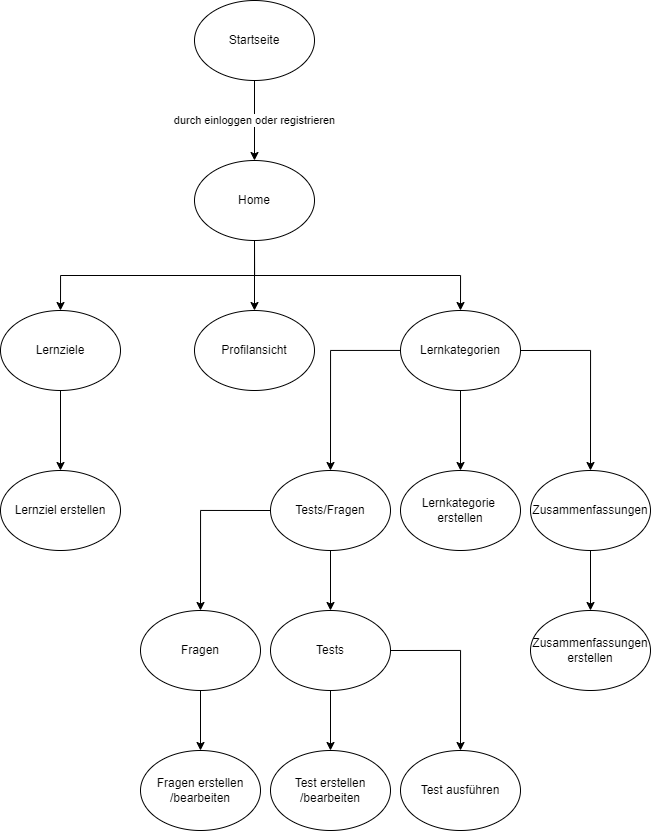
\includegraphics[width=0.8\textwidth]{images/diagramme/Seitenhierarchie.png}
  \caption{Die Seitenhierarchie in LearnAhead}
  \label{fig:UseCaseDiagramm1}
\end{figure}

\newpage
\subsubsection{UI-Mockups}

\begin{figure}[htbp]
  \centering
  \begin{subfigure}[b]{0.45\linewidth}
    \centering
    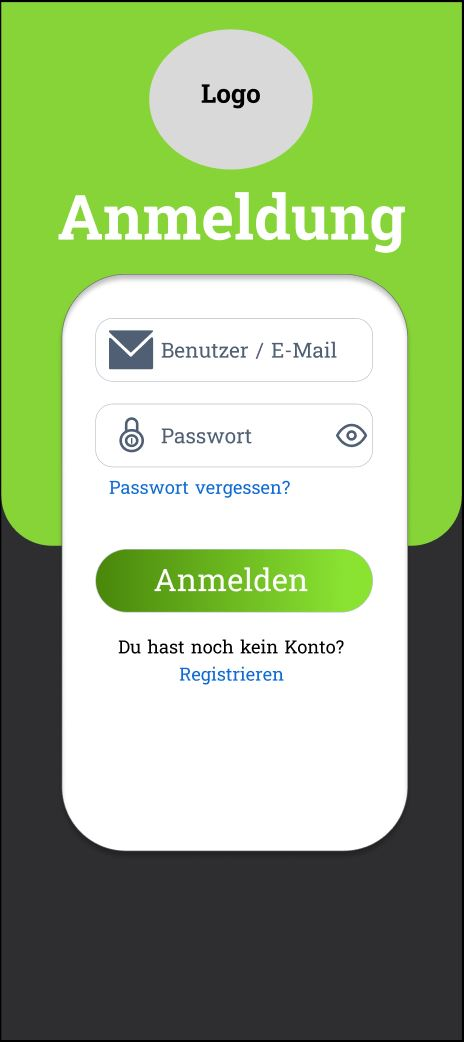
\includegraphics[width=\linewidth]{images/Mockups/Login.JPG}
    \caption{Login-Screen}
    \label{fig:login-screen}
  \end{subfigure}
  \hfill
  \begin{subfigure}[b]{0.45\linewidth}
    \centering
    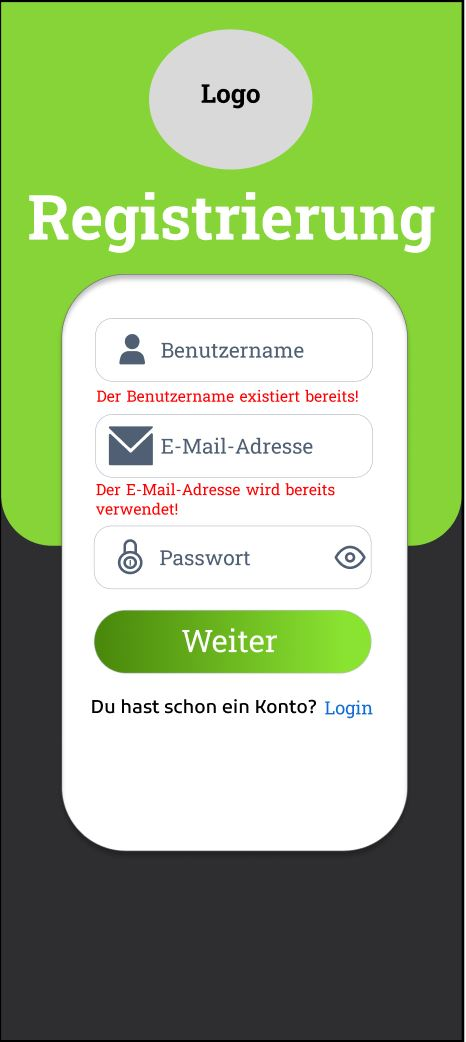
\includegraphics[width=\linewidth]{images/Mockups/Registrierung.JPG}
    \caption{Registrierung}
    \label{fig:registrierung}
  \end{subfigure}
  \caption{Login und Registrierung}
\end{figure}

\newpage

\begin{figure}[htbp]
  \centering
  \begin{subfigure}[b]{0.45\linewidth}
    \centering
    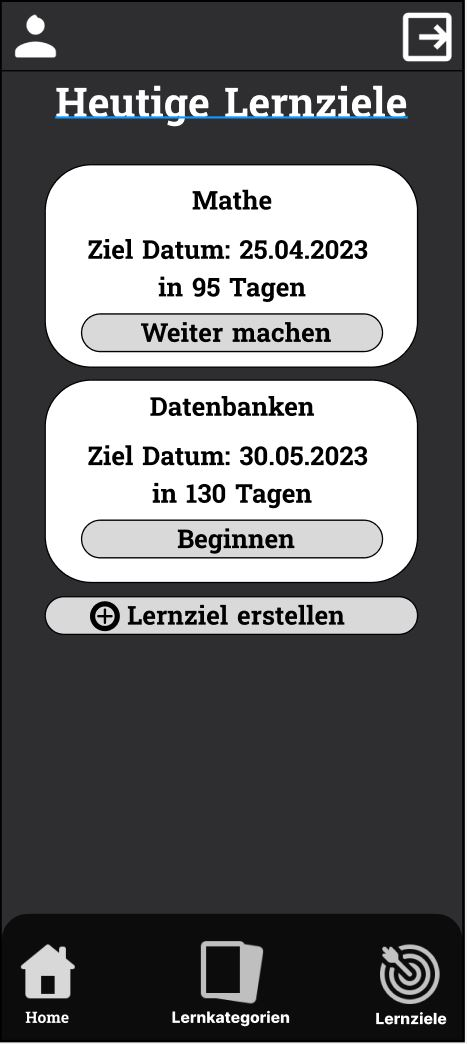
\includegraphics[width=\linewidth]{images/Mockups/Home.JPG}
    \caption{Home-Screen}
    \label{fig:home-screen}
  \end{subfigure}
  \hfill
  \begin{subfigure}[b]{0.45\linewidth}
    \centering
    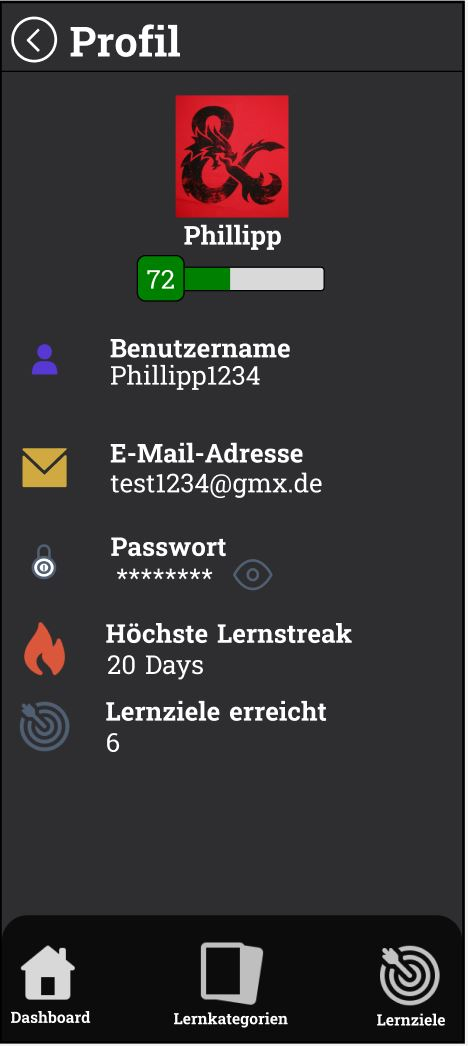
\includegraphics[width=\linewidth]{images/Mockups/Profile.JPG}
    \caption{Profilansicht}
    \label{fig:profilansicht}
  \end{subfigure}
  \caption{Home-Screen and Profilansicht}
\end{figure}

\newpage

\begin{figure}[htbp]
  \centering
  \begin{subfigure}[b]{0.45\linewidth}
    \centering
    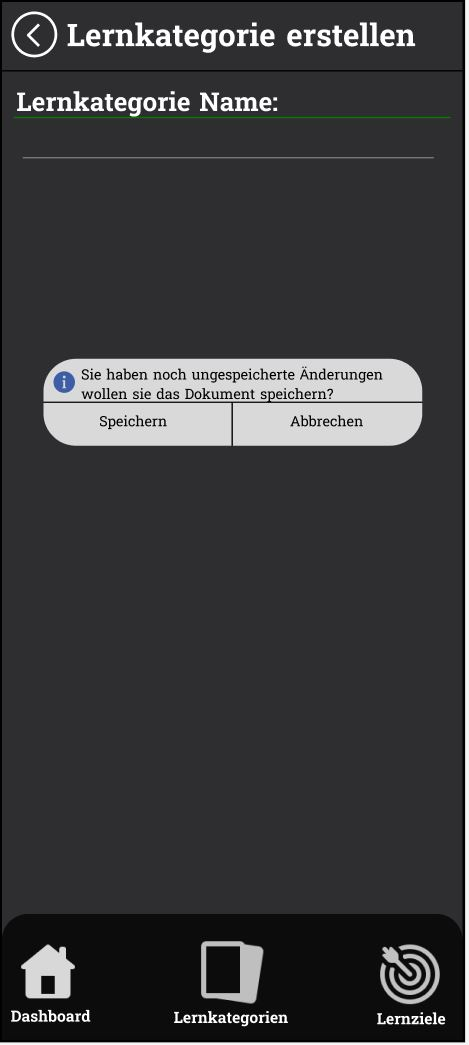
\includegraphics[width=\linewidth]{images/Mockups/createLernkategorie.JPG}
    \caption{Erstellen einer Lernkategorie}
    \label{fig:lernkategorie-create}
  \end{subfigure}
  \hfill
  \begin{subfigure}[b]{0.45\linewidth}
    \centering
    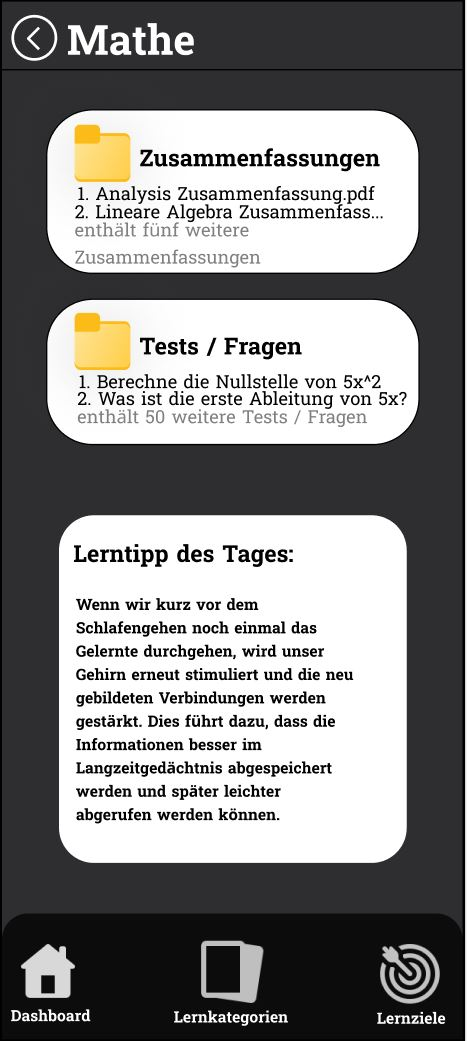
\includegraphics[width=\linewidth]{images/Mockups/Lernkategorie.JPG}
    \caption{Ansicht Lernkategorien}
    \label{fig:lernkategorie-ansicht}
  \end{subfigure}
  \caption{Erstellen einer Lernkategorie and Ansicht Lernkategorien}
  \label{fig:lernkategorie}
\end{figure}

\newpage

\begin{figure}[htbp]
  \centering
  \begin{subfigure}[b]{0.45\linewidth}
    \centering
    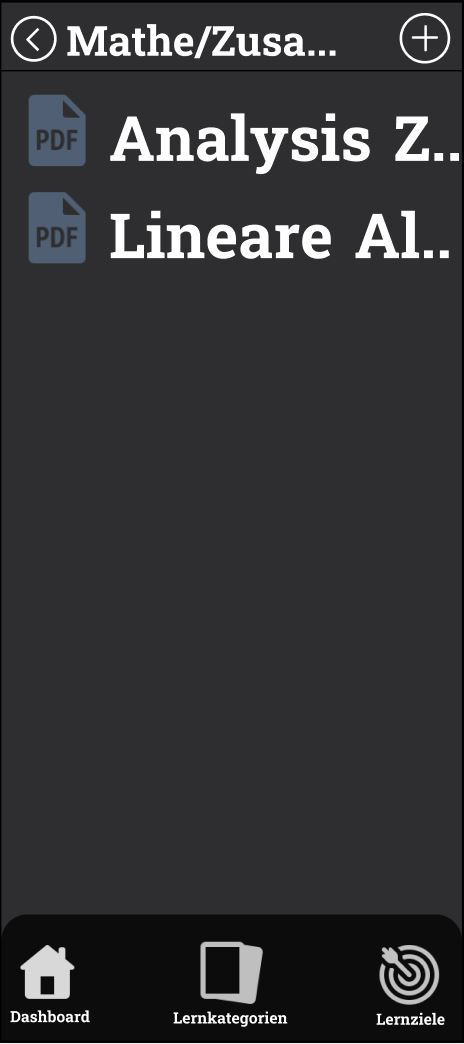
\includegraphics[width=\linewidth]{images/Mockups/Summaries.JPG}
    \caption{Ansicht Zusammenfassungen}
    \label{fig:zusammenfassungen-ansicht}
  \end{subfigure}
  \hfill
  \begin{subfigure}[b]{0.45\linewidth}
    \centering
    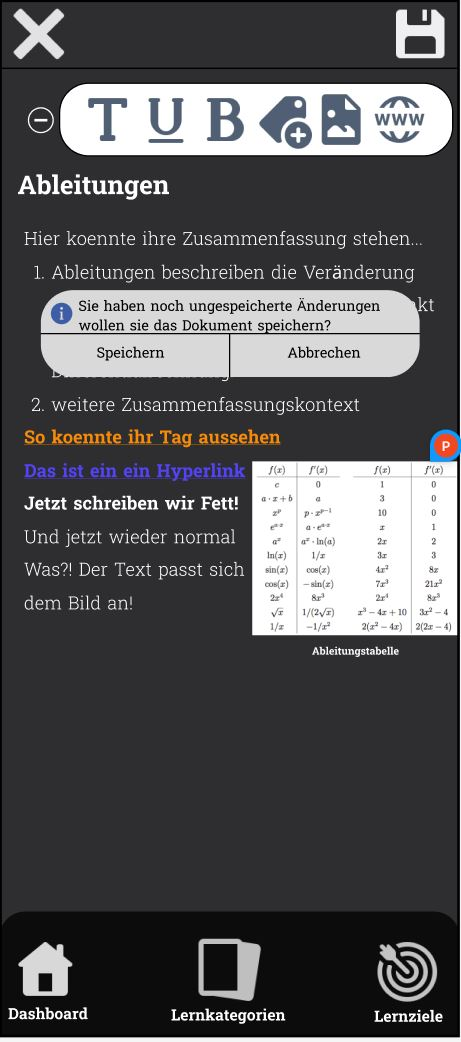
\includegraphics[width=\linewidth]{images/Mockups/Summaries_Look.JPG}
    \caption{Erstellen einer Zusammenfassung}
    \label{fig:zusammenfassungen-erstellen}
  \end{subfigure}
  \caption{Ansicht Zusammenfassungen and Erstellen einer Zusammenfassung}
  \label{fig:zusammenfassungen}
\end{figure}

\newpage

\begin{figure}[htbp]
  \centering
  \begin{subfigure}[b]{0.45\linewidth}
    \centering
    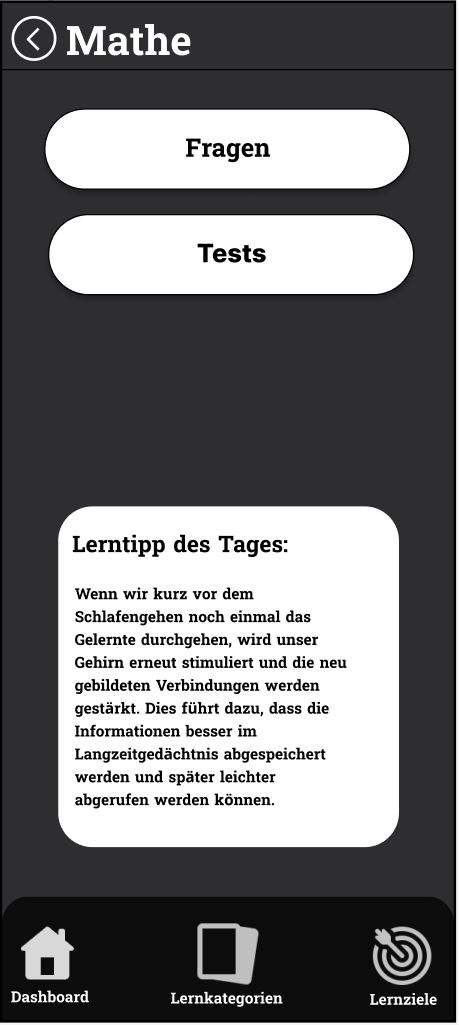
\includegraphics[width=\linewidth]{images/Mockups/FragenTests.JPG}
    \caption{Ansicht Fragen und Tests}
    \label{fig:fragen-tests-ansicht}
  \end{subfigure}
  \hfill
  \begin{subfigure}[b]{0.45\linewidth}
    \centering
    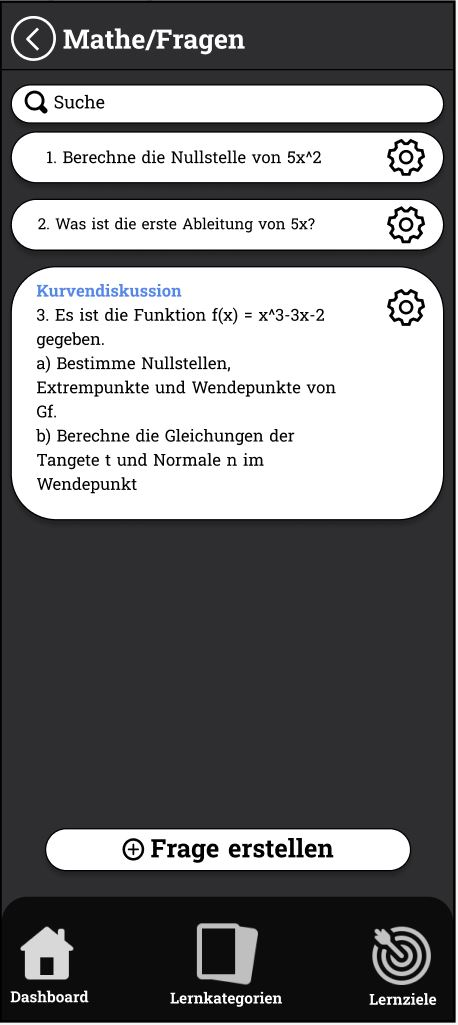
\includegraphics[width=\linewidth]{images/Mockups/Fragen.JPG}
    \caption{Ansicht Fragen}
    \label{fig:fragen-ansicht}
  \end{subfigure}
  \caption{Ansicht Fragen und Tests and Ansicht Fragen}
  \label{fig:fragen-tests}
\end{figure}

\newpage

\begin{figure}[htbp]
  \centering
  \begin{subfigure}[b]{0.45\linewidth}
    \centering
    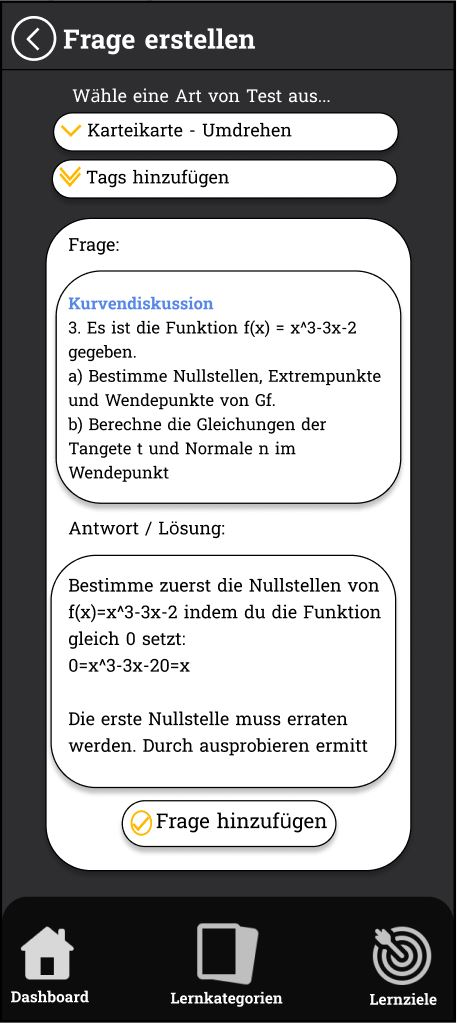
\includegraphics[width=\linewidth]{images/Mockups/FrageErstellen.JPG}
    \caption{Erstellen einer Frage}
    \label{fig:frage-erstellen}
  \end{subfigure}
  \hfill
  \begin{subfigure}[b]{0.45\linewidth}
    \centering
    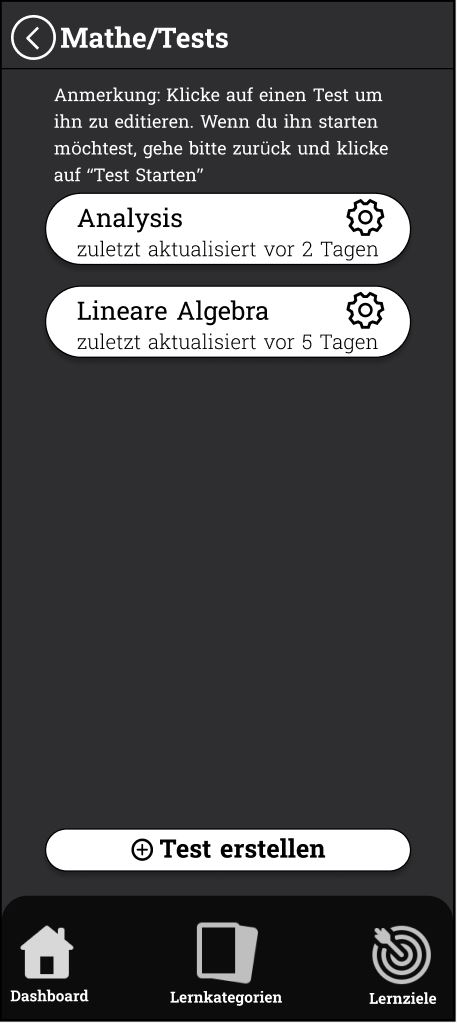
\includegraphics[width=\linewidth]{images/Mockups/Tests.JPG}
    \caption{Ansichts Tests}
    \label{fig:tests-ansicht}
  \end{subfigure}
  \caption{Erstellen einer Frage and Ansichts Tests}
  \label{fig:frage-tests}
\end{figure}

\newpage

\begin{figure}[htbp]
  \centering
  \begin{subfigure}[b]{0.45\linewidth}
    \centering
    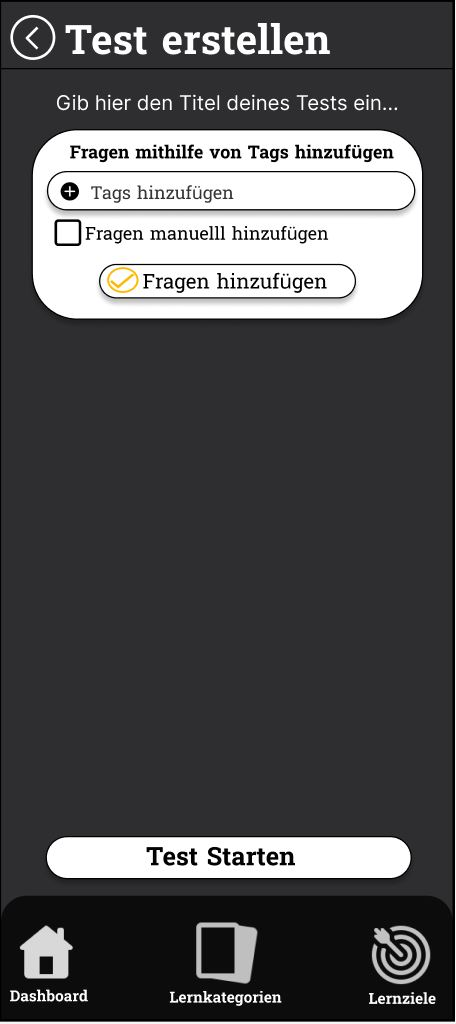
\includegraphics[width=\linewidth]{images/Mockups/TestErstellen.JPG}
    \caption{Erstellen eines Tests}
    \label{fig:test-erstellen}
  \end{subfigure}
  \hfill
  \begin{subfigure}[b]{0.45\linewidth}
    \centering
    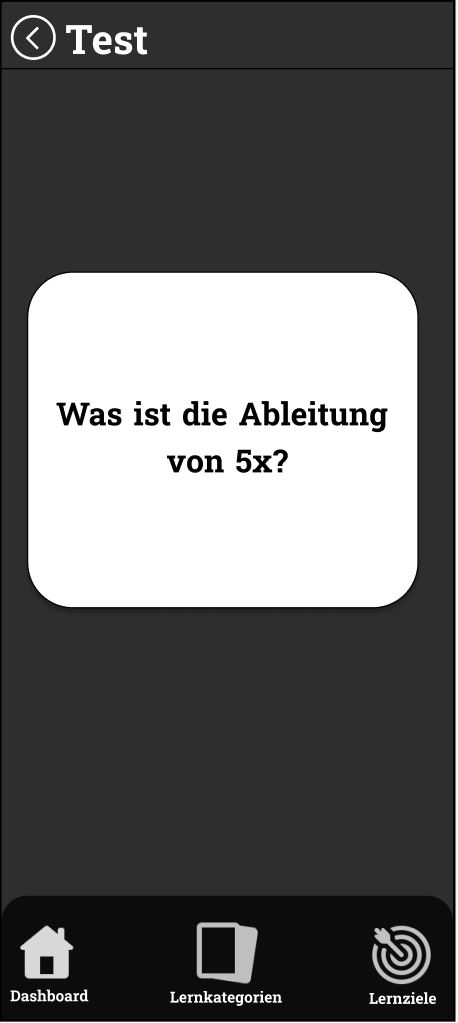
\includegraphics[width=\linewidth]{images/Mockups/TestFrage.JPG}
    \caption{Ansicht einer Frage innerhalb eines Tests}
    \label{fig:test-frage}
  \end{subfigure}
  \caption{Test}
\end{figure}

\newpage

\begin{figure}[htbp]
  \centering
  \begin{subfigure}[b]{0.45\linewidth}
    \centering
    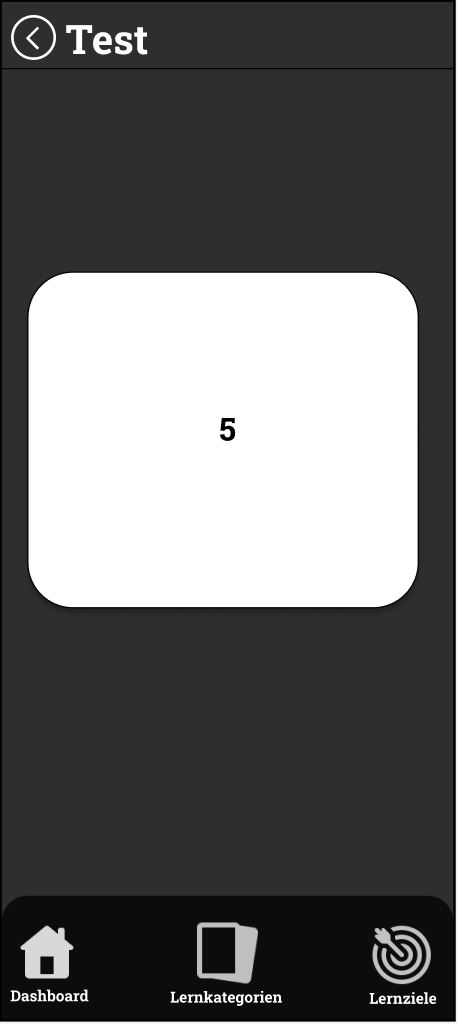
\includegraphics[width=\linewidth]{images/Mockups/TestAntwort.JPG}
    \caption{Ansicht einer Antwort innerhalb eines Tests}
    \label{fig:test-antwort}
  \end{subfigure}
  \hfill
  \begin{subfigure}[b]{0.45\linewidth}
    \centering
    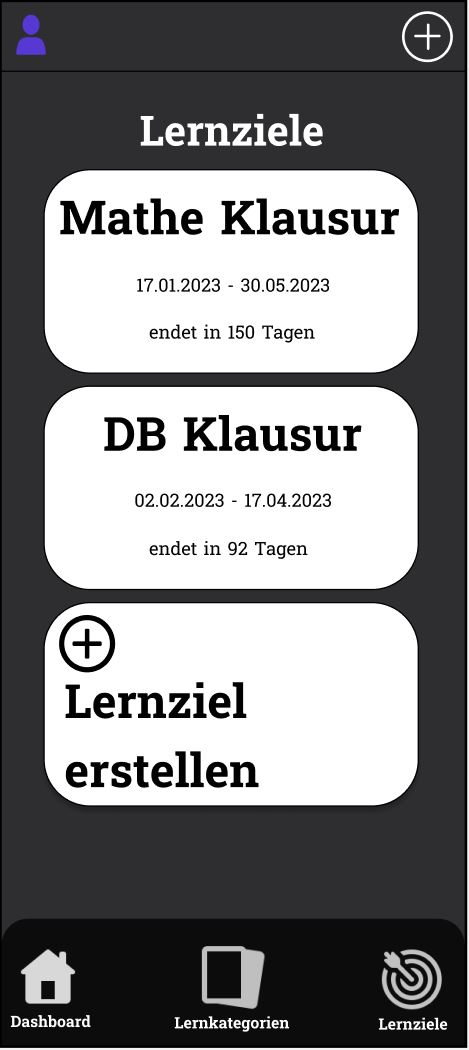
\includegraphics[width=\linewidth]{images/Mockups/Lernziele.JPG}
    \caption{Ansicht Lernziele}
    \label{fig:lernziele}
  \end{subfigure}
  \caption{Test}
\end{figure}

\newpage

\begin{figure}[H]
  \centering
  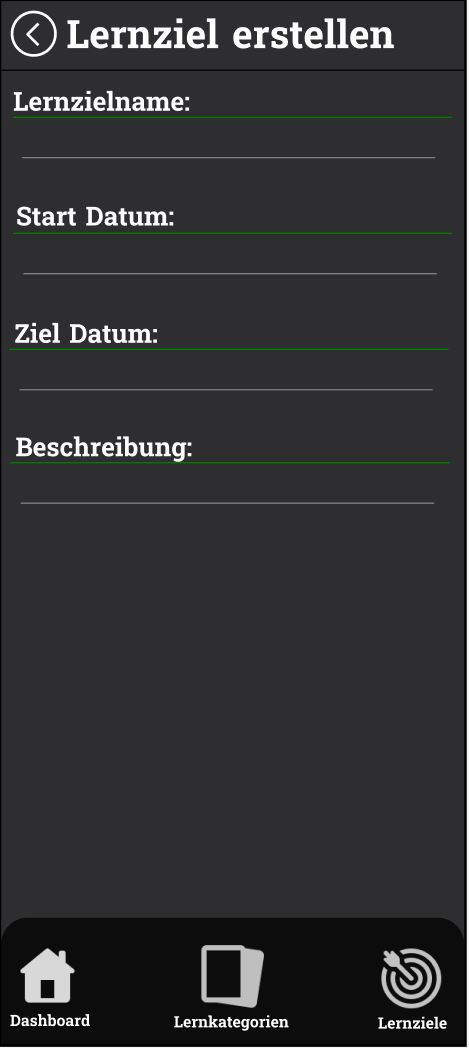
\includegraphics[width=0.5\linewidth]{images/Mockups/LernzielErstellen.JPG}
  \caption{Erstellen eines Lernziels}
  \label{fig:lernziel-erstellen}
\end{figure}

\newpage

\subsection{Flow-Chart-Diagramm}
Die Interaktion des Users mit der App wird in dem Flow-Chart-Diagramm grob dargestellt. Hierbei ist noch zu erwähnen, dass die Farbe Grün für den Anfang und das Ende steht. Die Farbe Blau steht für die wichtigsten Seiten, die der User besuchen kann. Die Farbe Orange steht für die verschiedenen Aktionen, die der User ausführen kann. Die Farbe Gelb steht für die hauptsächliche Interaktion mit der App (z.B. das Wechseln der Seiten).
\begin{figure}[H]
  \centering
  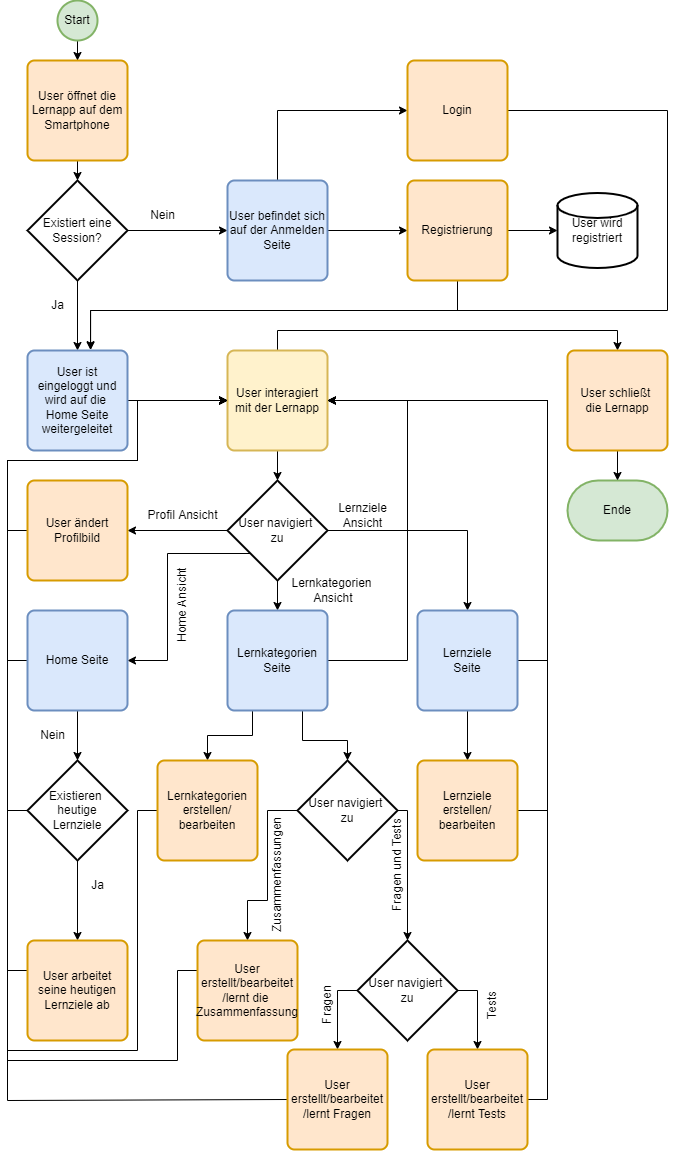
\includegraphics[width=0.66\textwidth]{images/diagramme/FlowChartDiagramm.png}
  \caption{Flow-Chart-Diagramm}
  \label{fig:FlowChart}
\end{figure}\noindent